% ------------------------------ Related Studies -----------------------------

\section{Related Studies}

\begin{comment}
    For avoiding plagiarism, citations should be used for all referred texts particularly here and other parts of the document using appropriate numbers within square bracket for all mapped references under \textbf{References} section. You should check any standard journal paper for typical use of citations.     
\end{comment}

\vspace{-2em}

\begin{table}[H]
    \centering
    \label{tab:related_studies}
    \begin{tabularx}{\textwidth}{|p{3.5cm}|X|}
    \hline
    \textbf{Study} & \textbf{Summary} \\ \hline
    Choudhury et al. (2013) & Explored the predictive capabilities of social media content in identifying depression by analyzing Twitter data. They discovered that specific linguistic patterns (e.g., negative emotion words) correlated strongly with self-reported depressive symptoms \cite{Choudhury2013PredictingDV}. \\ \hline
    Guntuku et al. (2017) & Conducted an integrative review which synthesized various methodologies highlighted that social media platforms are rich sources of data, revealing critical information about users' mental health \cite{Guntuku2017DetectingDA}. \\ \hline
    Mathur et al. (2022) & Provided a systematic review analysing machine learning techniques for mental health detection using social media data, leveraging both individual assessments and broader epidemiological studies \cite{Mathur2022MentalHC}. \\ \hline
    Nadeem (2016) & Investigated depression identification on Twitter by developing algorithms to discern emotional cues in tweets revealing that simple text analysis could lead to improvements in identifying mental risks \cite{nadeem2016identifying}. \\ \hline
    AlSagri and Ykhlef (2020) & Introduced a machine learning–based approach for depression detection on Twitter that combined both content and activity features. Their work demonstrated that a fusion of linguistic and behavioral analysis can enhance the accuracy of depression identification \cite{alsagri2020machine}. \\ \hline
    Vaishnavi et al. (2022) & Examined various machine learning algorithms for predicting mental health illnesses using social media posts. Their findings emphasized that certain algorithms outperform others in classifying mental health conditions, underlining the importance of algorithm selection \cite{Vaishnavi_2022}. \\ \hline
    Safa et al. (2023) & Presented a roadmap for predicting mental health using social media, highlighting ongoing challenges such as ethical considerations and data privacy. They stressed the need for a robust ethical framework in research that leverages social media data \cite{safa2023predictingmentalhealthusing}. \\ \hline
    Ensemble learning using transformers for NLP & Provided a comprehensive review of transformer models (BERT, XLNet, RoBERTa, GPT-2, ALBERT) across multiple NLP tasks. The study introduced ensemble learning with these models and demonstrated that ensemble approaches can significantly improve performance over single classifier methods \cite{Zhang_2024}. \\ \hline
    Ensemble hybrid model for depression detection & Proposed an ensemble hybrid model combining SVM and MLP to improve depression prediction accuracy. Addressing class imbalance with SMOTE and cluster sampling, the model achieved an accuracy of 99.39\% and an F1-score of 99.51\%, outperforming previous approaches \cite{Saha2024}. \\ \hline
    Single classifier vs. ensemble ML approaches & Explored various machine learning techniques to predict mental health issues using survey responses from OSMI. The study compared single classifiers (e.g., Logistic Regression, Gradient Boosting, Neural Networks, KNN, SVM) with ensemble approaches, finding that Gradient Boosting achieved the highest accuracy (88.80\%), followed by Neural Networks (88.00\%), and that the ensemble classifier achieved 85.60\% accuracy \cite{Chung_2023}. \\ \hline
\end{tabularx}
\end{table}


% ----- add pre frame study

\begin{figure}[H]  
    \centering
    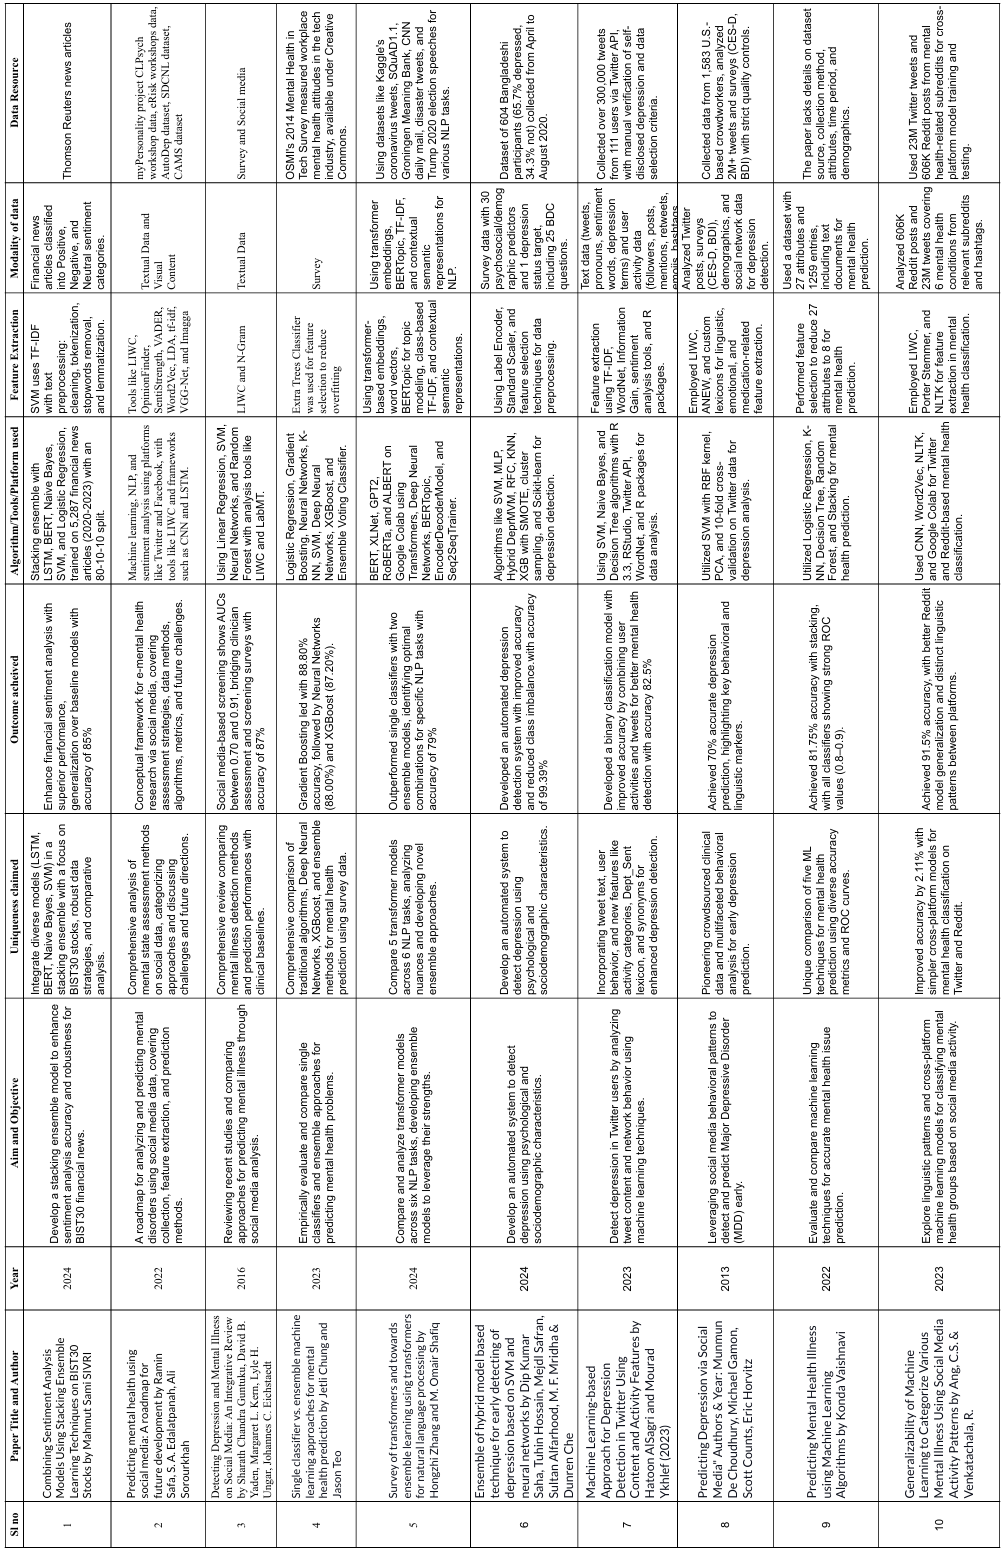
\includegraphics[width=0.95\textwidth]{Images/preframe-study.png}  
    \caption*{Pre frame study review}
    \label{Preframe Study Review}  % Label for referencing the figure
\end{figure}


\pagebreak
% ----------------------------- Related Studies End --------------------------
